\setlength{\tabcolsep}{2pt}
\newcommand{\sampletbl}[2]{
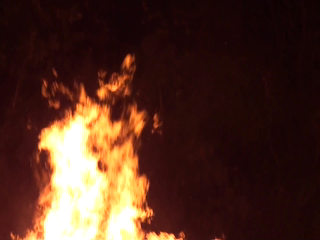
\includegraphics[width=0.5in]{stablefn/results/#1-#2/fr_00000.png} &
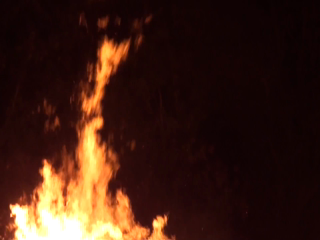
\includegraphics[width=0.5in]{stablefn/results/#1-#2/fr_00010.png} &
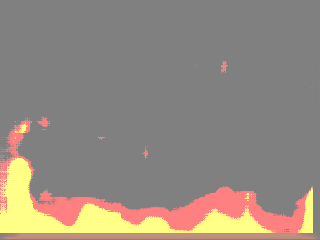
\includegraphics[width=0.5in]{stablefn/results/#1-#2/fr_00020.png} &
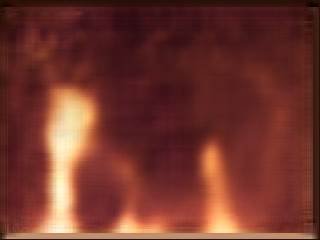
\includegraphics[width=0.5in]{stablefn/results/#1-#2/fr_00030.png} &
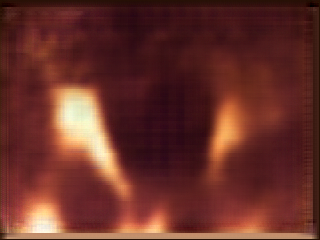
\includegraphics[width=0.5in]{stablefn/results/#1-#2/fr_00040.png} &
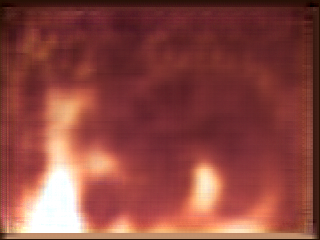
\includegraphics[width=0.5in]{stablefn/results/#1-#2/fr_00050.png} &
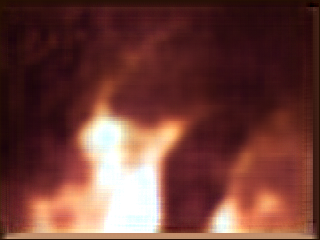
\includegraphics[width=0.5in]{stablefn/results/#1-#2/fr_00100.png} &
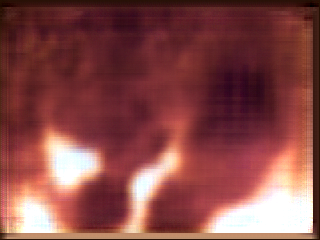
\includegraphics[width=0.5in]{stablefn/results/#1-#2/fr_00150.png} &
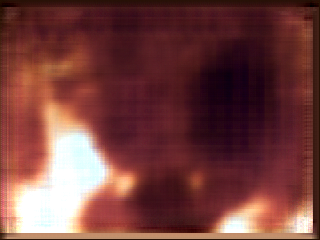
\includegraphics[width=0.5in]{stablefn/results/#1-#2/fr_00200.png} &
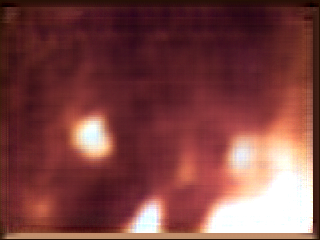
\includegraphics[width=0.5in]{stablefn/results/#1-#2/fr_00250.png}
}

\begin{tikzpicture}
    \begin{groupplot}[
        group style={
            group name=my plots,
            group size=5 by 1,
            horizontal sep=12pt
        },
        axis on top,% ----
        width=1.2in,
        height=1.2in,
        scale only axis,
        enlargelimits=false,
        xmin=0,
        xmax=1,
        ymin=0,
        ymax=1,
        axis x line*=bottom, axis y line*=left,
        ]

    \nextgroupplot[title={Stable Model Run 1},
    ytick={.1, 1},
    yticklabels={-2,18},
    xtick={.15, 1},
    xticklabels={$-10$,15}]
    \addplot[
        yticklabels={,,},
        xticklabels={,,}] graphics[xmin=-0.17,ymin=-0.17,xmax=1.17,ymax=1.17] {./stablefn/results/bonfire-exp27r-1e-5-1231132/trajmodel.png};

    \nextgroupplot[title={Stable Model Run 2},
    ytick={.1, 1},
    yticklabels={0,$20$},
    xtick={.15, 1},
    xticklabels={$0$,25}]
\addplot[] graphics[xmin=-0.17,ymin=-0.17,xmax=1.17,ymax=1.17] {./stablefn/results/bonfire-exp27r-1e-5-1238886/trajmodel.png};

    \nextgroupplot[title={Stable Model Run 3},
    ytick={.1, 1},
    yticklabels={-10,8},
    xtick={.1, .8},
    xticklabels={-5,15}]
    ]
    \addplot[] graphics[xmin=-0.17,ymin=-0.17,xmax=1.17,ymax=1.17] {./stablefn/results/bonfire-exp27r-1e-5-main/trajmodel.png};

    \nextgroupplot[title={Naive Model},
    ytick={.1, 1},
    yticklabels={0,},
    xtick={.1, 1},
    xticklabels={$-2 \times 10^{30}$,0},
        extra y tick labels={$1.2 \times 10^{30}$},
        extra y ticks={1.0},
        extra y tick style={y tick label style={right, xshift=0.25em}},]
    \addplot[] graphics[xmin=-0.17,ymin=-0.17,xmax=1.17,ymax=1.17] {./stablefn/results/bonfire-bad2/trajmodel.png};
    
    \nextgroupplot[
        ytick={0,1},
        yticklabels={0,300},
        ylabel={steps},
        width=.075in,
        axis line style={draw=none}, tick style={draw=none}, xticklabel=\empty, every axis y label/.style={at={(current axis.west)},rotate=90,yshift=-3mm,xshift=1mm},
        y tick label style={right, xshift=0.25em}]

    \addplot[] graphics[xmin=0,ymin=0,xmax=1,ymax=1] {./stablefn/viridis.png};

\end{groupplot}
\end{tikzpicture}
\begin{tabular}{r|cccccc|cccc}
Stable & \multicolumn{10}{c}{Frame Number} \\
Model & $0$ & ${10}$ & ${20}$ & ${30}$ & ${40}$ & ${50}$ & ${100}$ & ${150}$ & ${200}$ & ${250}$ \\
Run 1 &\sampletbl{bonfire}{exp27r-1e-5-main} \\
Run 2 &\sampletbl{bonfire}{exp27r-1e-5-1231132} \\
Run 3 &\sampletbl{bonfire}{exp27r-1e-5-1238886} \\
\shortstack{Naive\\Model} &
\sampletbl{bonfire}{bad2}
% \\ \shortstack{Sample\\Video} &    \sampletbl{bonfire}{sample}
\end{tabular}
